\documentclass[
  11pt,
  letterpaper,
   addpoints,
   %answers
  ]{exam}

% Carga el preámbulo localizado en la carpeta superior
\NeedsTeXFormat{LaTeX2e}[2023/04/30]

% Provide the name of your page, the date it was last updated, and a comment about what it's used for
\ProvidesPackage{../exercise-preamble}[2023/04/30 Prof. Cassanelli custom LaTeX style]

% \usepackage{printlen}
% \uselengthunit{in}\printlength{\textwidth}

% PACKAGES
\usepackage[dvipsnames]{xcolor}

\usepackage{graphicx}
\graphicspath{{../figures}}
\usepackage{amsmath,amsthm,amssymb,mathtools,mathrsfs}
\usepackage{commath}
\usepackage{upgreek}
\usepackage{cancel}
\usepackage{enumerate}
\usepackage[font=small]{caption}
\usepackage[normalem]{ulem}
\usepackage{steinmetz}
\usepackage{enumitem}
\usepackage[left=1.5cm, right=1.5cm, top=1cm]{geometry}
\usepackage{wrapfig}

% REFERENCES AND OTHERS
\usepackage{../aas_macros}
\usepackage{natbib}
\bibpunct{(}{)}{;}{a}{}{,}

\usepackage{tikz}
\usepackage{tikz-3dplot}
\usepackage{circuitikz}
\usepackage{pgfplots}
\pgfplotsset{compat=1.15}
\usepgfplotslibrary{smithchart}
\usetikzlibrary{
  decorations.pathmorphing,
  decorations.markings,
  calc,
  patterns,
  decorations,
  angles,
  quotes,
  ext.topaths.arcthrough,
  shapes
  }

\usepackage{siunitx}
\sisetup{
    range-phrase=\text{--},
    range-units=single,
    separate-uncertainty=true,
    print-unity-mantissa=false
    }
\DeclareSIUnit{\gauss}{G}
\DeclareSIUnit{\jansky}{Jy}

\newcommand{\iu}{\mathrm{i}\mkern1mu}
\newcommand{\ju}{\mathrm{j}\mkern1mu}
\newcommand{\euler}{\mathrm{e}}
\newcommand{\exponential}[1]{\mathrm{exp}\left[#1\right]}
\newcommand{\uvec}[1]{\widehat{\mathbf{#1}}}
\newcommand{\uvecs}[1]{\boldsymbol{\widehat{#1}}}
\newcommand{\bvec}[1]{\boldsymbol{\mathcal{#1}}}

\usepackage{hyperref}
\hypersetup{
    % bookmarks=true,
    unicode=true,
    pdftoolbar=true,
    pdfmenubar=true,
    pdffitwindow=false,
    pdfstartview={FitH},
    pdftitle={EL3103},
    pdfauthor={Tomas Cassanelli},
    pdfcreator={Tomas Cassanelli},
    pdfnewwindow=true,
    colorlinks=true,
    linkcolor=Violet,
    citecolor=Violet,
    urlcolor=Violet
    }

% Exam document class
\renewcommand{\figurename}{Figura}
\renewcommand{\tablename}{Cuadro}
\pagestyle{empty}

\usepackage[spanish]{cleveref}

\crefname{question}{\protect{pregunta}}{\protect{preguntas}}
\Crefname{question}{\protect{Pregunta}}{\protect{Preguntas}}
\creflabelformat{question}{#2{#1}#3}

\renewcommand{\solutiontitle}{\noindent\textbf{Solución:}\par\noindent}
\bracketedpoints
\pointname{~puntos}

\endinput

% Paquetes locales
\usepackage{float}
\usepackage{booktabs} % para \toprule, \midrule, \bottomrule
\usepackage{xcolor} % para colores

% Macros locales
\newcommand{\Rel}{\mathfrak{R}} % símbolo para la reluctancia

\begin{document}

\noindent
\begin{minipage}{0.47\textwidth}

\includegraphics[width=\textwidth]{../fcfm_die}
\end{minipage}
\begin{minipage}{0.53\textwidth}
\begin{center}
\large\textbf{Análisis de Sistemas Dinámicos y Estimación} (EL3204-1) \\
\large\textbf{Ejercicio 1} \\
\normalsize Prof.~ Marcos Orchard - Sebastián Espinosa.\\
\normalsize Prof.~Aux.~Erik Sáez
\end{center}
\end{minipage}

\vspace{0.5cm}
\noindent\fbox{%
  \parbox{\dimexpr\linewidth-2\fboxsep-2\fboxrule\relax}{%
    	\textbf{Instrucciones:} La tarea se puede realizar en grupos de 3 con un plazo máximo hasta el viernes 17 de Octubre; no se aceptarán atrasos. El formato deberá ser entregada escrita a mano o en tablet (letra legible), además de entrega virtual de los códigos que utilicen.
  }%
}

\vspace{.85cm}

    %%%%%%%%%%%%%%%%%%%%%%%%%%%
    Considere el sistema electromecánico de la figura~\ref{fig:relay}, que modela de forma simplificada el funcionamiento de un relé electromagnético utilizado en el sistema de control de un robot industrial para el ensamblaje de componentes electrónicos de precisión. Este dispositivo consta de un núcleo de hierro de sección transversal $A$ en el cual se induce flujo magnético mediante una bobina de $N$ vueltas. El relé controla actuadores neumáticos que operan las pinzas del robot, donde la precisión y eficiencia energética son críticas para la operación. Para este estudio, usted podrá modificar el voltaje de excitación $e(t)$ y analizará cómo el entrehierco modula la inductancia $L(x)$, la fuerza de atracción magnética y la dinámica de conmutación del sistema.\\

    \noindent\fbox{\parbox{0.92\linewidth}{\textbf{Nota:} Considere que el movimiento de la armadura móvil ocurre únicamente en una dirección (sobre el eje $x$), es decir, el desplazamiento es unidimensional.}}

\begin{figure}[h!]
  \centering
  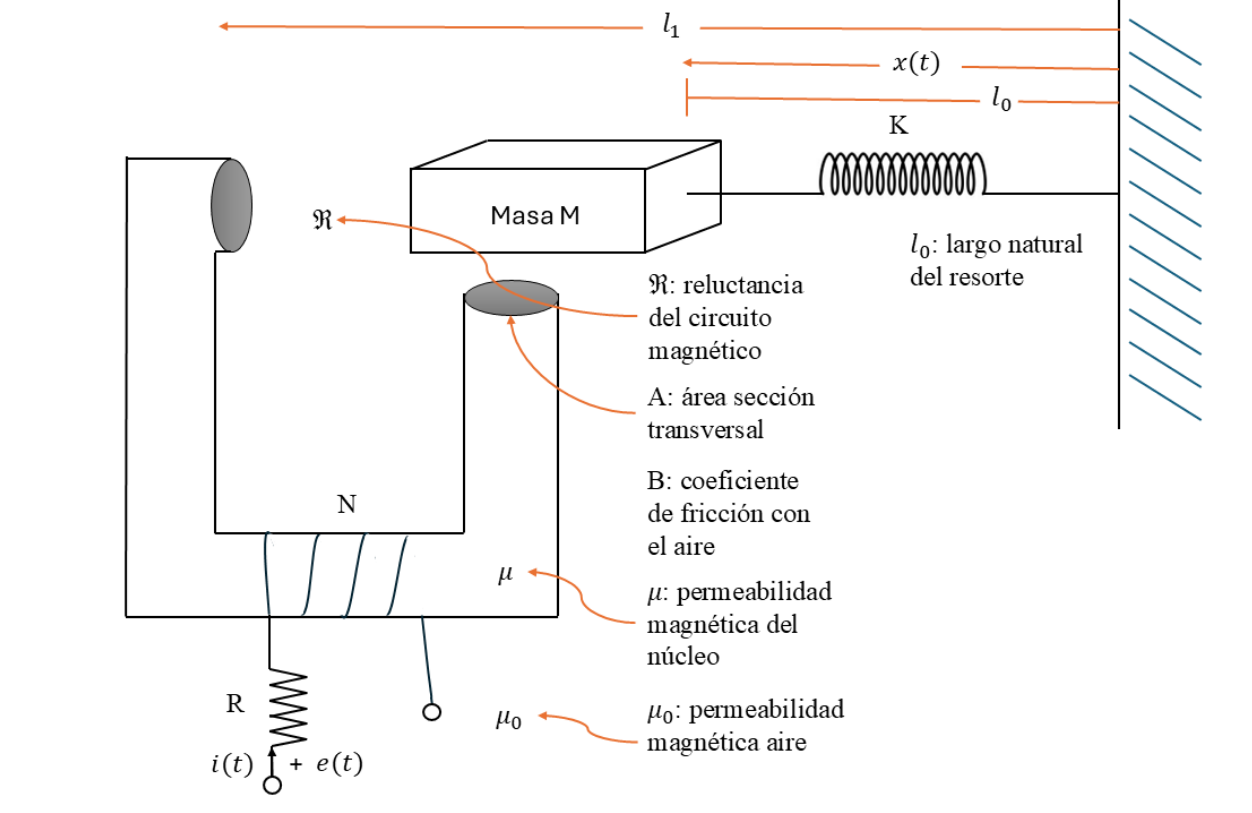
\includegraphics[width=0.8\textwidth,keepaspectratio]{Ejercicio_1_1}
  \caption{Sistema electromecánico del relé electromagnético mostrando la armadura móvil de masa $M$, el resorte de constante $K$, el entrehierro variable $x(t)$, y el circuito eléctrico equivalente con resistencia $R$ y voltaje de excitación $e(t)$.}
  \label{fig:relay}
\end{figure}

Los parámetros del sistema, junto con sus respectivas unidades de medida, se detallan en la Tabla~\ref{tab:variables}.

\begin{table}[H]
  \centering
  \caption{Variables y parámetros del sistema}
  \label{tab:variables}
  \small
  \begin{tabular}{@{}c p{9.5cm} c@{}}
    \toprule
    \textbf{Variable/Parámetro} & \textbf{Definición} & \textbf{Unidad} \\
    \midrule
    $x(t)$      & Posición de la armadura móvil entre $l_0$ y $l_1$ & m \\
    $i(t)$      & Corriente por la bobina                           & A \\
    $L(x)$      & Inductancia de la bobina                          & H \\
  $\Rel$      & Reluctancia del circuito magnético                & A/Wb (1/H) \\
    $e(t)$      & Voltaje en la bobina                              & V \\
    $M$         & Masa de la pieza                                  & kg \\
    $K$         & Coeficiente de rigidez del resorte                & N/m \\
    $B$         & Coeficiente de fricción viscosa del aire          & N/(m/s) \\
    $R$         & Resistencia eléctrica de la bobina                & $\Omega$ \\
    $A$         & Área de la sección transversal del núcleo         & m$^2$ \\
    $\mu$       & Permeabilidad magnética del núcleo                & H/m \\
    $\mu_0$     & Permeabilidad magnética del aire                  & H/m \\
    $N$         & Número de espiras de la bobina                    & -- \\
    \bottomrule
  \end{tabular}
\end{table}

Para el análisis electromagnético del sistema, es fundamental comprender la distribución del flujo magnético y las reluctancias involucradas. La fuerza magnetomotriz generada por la bobina está dada por $F_m = N \cdot i(t)$. Aplicando la ley de Ampère para un circuito magnético cerrado, se establece que:
\begin{align}
  N \cdot i = H_n \cdot l_n + H_g \cdot l_g  = \frac{B_n}{\mu} \cdot l_n + \frac{B_g}{\mu_0} \cdot l_g .
\end{align}
donde $B_n$ y $l_n$ corresponden a la densidad de flujo magnético y la longitud promedio del camino en el núcleo de hierro, respectivamente. Por otra parte, $B_g$ y $l_g$ representan la densidad de flujo magnético en el entrehierro y su longitud. La geometría del núcleo magnético se ilustra detalladamente en la Figura~\ref{fig:core}.

\begin{figure}[h!]
  \centering
  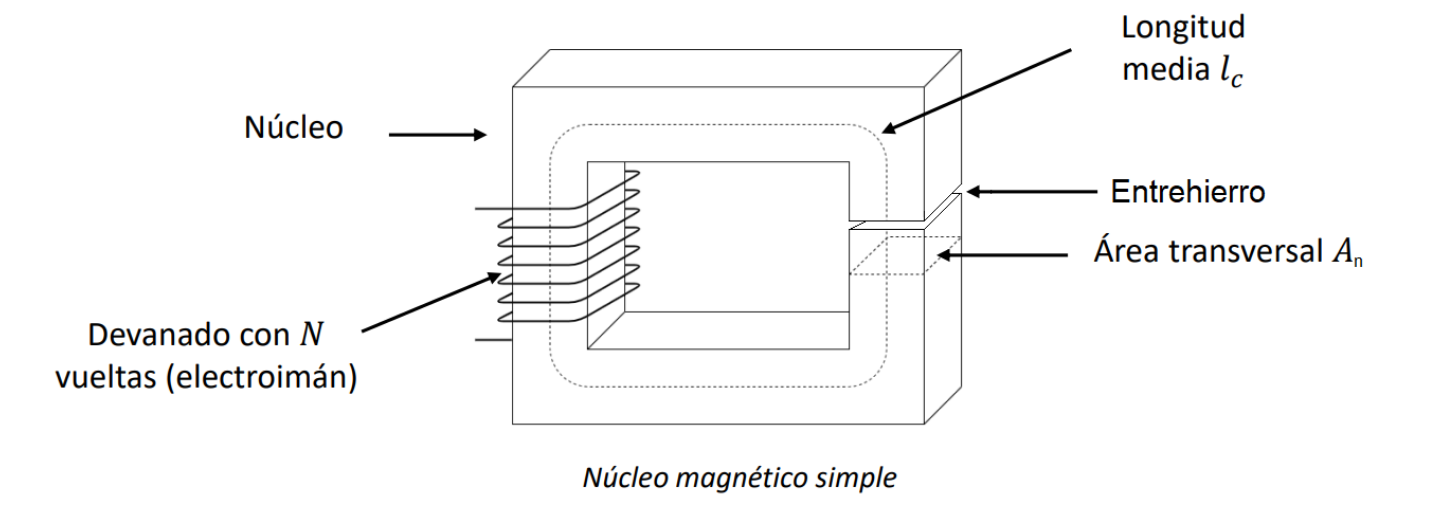
\includegraphics[width=0.85\textwidth,keepaspectratio]{Ejercicio_1_2}
  \caption{Diagrama del núcleo magnético simple mostrando el devanado de $N$ vueltas, el núcleo de hierro con longitud media $l_c$, el entrehierro de longitud variable, y el área transversal $A_n$ del flujo magnético.}
  \label{fig:core}
\end{figure}

El flujo magnético se define como la integral del campo magnético sobre la superficie transversal:
\begin{align}
  \int B_{n,g}\, \mathrm{d}s = \phi.
\end{align}
Considerando que el campo magnético es uniforme en la sección transversal del núcleo, se obtiene:
\begin{align}
  B_{n,g} = \frac{\phi}{A_n}.
\end{align}
Sustituyendo esta expresión en la ecuación de Ampère:
\begin{align}
  N \cdot i = \frac{\phi}{A_n \mu} \cdot l_n + \frac{\phi}{A_n \mu_0} \cdot l_g = \phi\!\left(\frac{l_n}{A_n \mu} + \frac{l_g}{A_n \mu_0}\right).
\end{align}

La reluctancia $\Rel$ es un parámetro fundamental que cuantifica la resistencia de un material al flujo magnético. Esta magnitud depende de la permeabilidad del material magnético ($\mu$), el área de la sección transversal ($A$) y la longitud del camino magnético ($l$):
\begin{align}
  \Rel = \frac{l}{A\,\mu}.
\end{align}
Aplicando este concepto al circuito magnético del relé:
\begin{align}
  N\,i &= \phi\,(\Rel_n + \Rel_g), \\
  \phi &= \frac{N\,i}{\Rel_n + \Rel_g}.
\end{align}

La relación entre el voltaje de la bobina y las variables electromagnéticas se establece mediante las ecuaciones fundamentales del electromagnetismo:
\begin{align}
  V_{\text{bobina}} = L\,\frac{\mathrm{d}i}{\mathrm{d}t} = N\,\frac{\mathrm{d}\phi}{\mathrm{d}t}.
\end{align}
Integrando esta ecuación con respecto al tiempo:
\begin{align}
  L\,i = N\,\phi.
\end{align}
Combinando con la expresión del flujo magnético:
\begin{align}
  L\,i = N\, \frac{N\, i}{\Rel_n + \Rel_g}
\end{align}
Definiendo la reluctancia total como $\Rel_{\text{total}} = \Rel_n + \Rel_g$ y despejando la inductancia:
\begin{align}
  L = \frac{N^2}{\Rel}
\end{align}

En el sistema analizado coexisten dos tipos principales de reluctancia: la reluctancia del entrehierro (debido al aire) y la reluctancia del núcleo de hierro. Dado que el hierro presenta una permeabilidad magnética mucho mayor que el aire, su reluctancia es considerablemente menor. Esta aproximación permite simplificar el análisis considerando que tanto el núcleo fijo como la armadura móvil están fabricados en hierro. El objetivo del estudio es analizar la dinámica del movimiento de la armadura de masa $M$ y la corriente del sistema, respondiendo a las preguntas formuladas en las siguientes secciones.
\newpage
\hrulefill
\begin{center}
\textbf{Valores numéricos de los parámetros del sistema}
\end{center}

\begin{table}[h!]
  \centering
  \caption{Parámetros numéricos del sistema electromecánico del relé electromagnético utilizados para el análisis cuantitativo, simulaciones y diseño del observador. Estos valores representan configuraciones típicas encontradas en aplicaciones industriales de precisión.}
  \label{tab:parametros-numericos}
  \begin{tabular}{@{}c c@{}}
    \toprule
    \textbf{Parámetro} & \textbf{Valor} \\
    \midrule
    $l_1$ & $0.03\,[\mathrm{m}]$ \\
    $l_0$ & $0.02\,[\mathrm{m}]$ \\
    $N$   & $200$ espiras \\
    $a$   & $0.0001\,[\mathrm{m}^2]$ \\
    $\mu_0$ & $4\pi \times 10^{-7}\,[\mathrm{H/m}]$ \\
    $K$   & $0.01\,[\mathrm{N/m}]$ \\
    $B$   & $0.00000001\,[\mathrm{N/(m/s)}]$ \\
    \bottomrule
  \end{tabular}
\end{table}
\begin{questions}
\question \textbf{Modelamiento matemático}
\begin{enumerate}
  \item \textcolor{blue}{\textbf{[0.15 pts]}} Establezca de forma clara todas las hipótesis simplificatorias del sistema. Considere que la Figura~\ref{fig:core} no tiene errores y, por tanto, si considera que falta algún dato o parámetro indique cómo abordará esto para que el modelo tenga sentido. Además, se aconseja investigar sobre transformadores ideales.

  \item \textcolor{blue}{\textbf{[0.3 pts]}} Formule el modelo matemático. Para ello deberá encontrar dos ecuaciones; una para la parte eléctrica del sistema y la otra para la parte mecánica del mismo. \emph{Hint}: la fuerza magnética interactúa con la pieza móvil según $F_m = \frac{1}{2} i^2\, \frac{\mathrm{d}L}{\mathrm{d}x}$. Además, si el valor $L$ de una inductancia varía con el tiempo a través de una función $g(t)$, entonces, el voltaje en esa inductancia será $V_{\text{ind}} = \frac{\mathrm{d}}{\mathrm{d}t}\left[L(g(t)) \cdot i(t)\right]$.

  \item \textcolor{blue}{\textbf{[0.25 pts]}} En base al contexto del problema, indique las variables que corresponden a la/s entrada/s, salida/s y variable/s de estado del sistema. Replantee el modelo como un sistema matricial de la forma $\dot{\vec{X}}(t) = \vec{F}\big(\vec{X}(t), u(t)\big)$ con su respectiva salida $\vec{Y}(t) = C \cdot \vec{X}(t)$, donde $\vec{X}(t)$ representa el vector de estados, $C$ la matriz de salida y $u(t)$ la/s entrada/s al sistema.

  \item \textcolor{blue}{\textbf{[0.15 pts]}} Encuentre el/los estado/s de equilibrio del sistema no lineal.

  \item \textcolor{blue}{\textbf{[0.15 pts]}} Encuentre las ecuaciones del/los punto/s de operación que asegura que la pieza móvil esté en una posición arbitraria $x_0$. Luego, exprese una única ecuación que involucre la posición de la pieza móvil y la entrada $u_0(t)$ (no es necesario despejar la posición de la pieza móvil).
\end{enumerate}

\question \textbf{Linealización-Laplace-MTE}

\begin{enumerate}
  \item \textcolor{blue}{\textbf{[0.3 pts]}} Linealice el sistema planteado en la pregunta anterior en torno a un punto de operación arbitrario $(\vec{X}(t_0), u(t_0))$ con tal de obtener la expresión $\dot{\vec{X}} = A \cdot \vec{X} + B \cdot u$, donde $A$ es la matriz de estado y $B$ la matriz de entrada.

  \item \textcolor{blue}{\textbf{[0.2 pts]}} Considere el sistema linealizado del primer punto. Evalúe el sistema en torno al estado de equilibrio que usted considere pertinente según lo que encontró en P1.4. \textbf{Importante:} Para las siguientes preguntas se considerará este sistema en particular.

  \item \textcolor{blue}{\textbf{[0.25 pts]}} Obtenga la MTE del sistema linealizado en torno al punto de equilibrio.

  \item \textcolor{blue}{\textbf{[0.25 pts]}} Obtenga la función de transferencia del sistema linealizado en torno al punto de equilibrio.
\end{enumerate}

\question \textbf{Determinación de estados}
\begin{enumerate}
  \item \textcolor{blue}{\textbf{[0.5 pts]}} Encuentre los estados cero del sistema linealizado alrededor del punto de equilibrio. Especifique claramente la definición usada y calcule los vectores de estado que satisfacen la condición de salida nula.

  \item \textcolor{blue}{\textbf{[0.5 pts]}} Encuentre los estados "tierra" (estados de reposo) del sistema linealizado alrededor del punto de equilibrio. Indique las condiciones iniciales asociadas si corresponde.
\end{enumerate}

\question \textbf{Polos, respuesta al impulso, RESC y RENC}
\begin{enumerate}
  \item \textcolor{blue}{\textbf{[0.2 pts]}} Determine los polos del sistema linealizado en torno al punto de equilibrio y comente su implicancia dinámica (estabilidad, oscilación, amortiguamiento).

  \item \textcolor{blue}{\textbf{[0.2 pts]}} Usando la función de transferencia del sistema linealizado, obtenga la respuesta al impulso en el dominio del tiempo y describa sus características principales.

  \item \textcolor{blue}{\textbf{[0.2 pts]}} Calcule la respuesta en estado cero (RESC) para el sistema linealizado en torno al punto de equilibrio ante una entrada arbitraria. Explique las hipótesis usadas.

  \item \textcolor{blue}{\textbf{[0.2 pts]}} Calcule la respuesta en estado (RENC) para condiciones iniciales arbitrarias del sistema linealizado. Presente la expresión en términos de la exponencial matricial si procede.

  \item \textcolor{blue}{\textbf{[0.2 pts]}} Exprese la solución completa del sistema linealizado alrededor del punto de equilibrio combinando RESC y RENC (solución general).
\end{enumerate}

\question \textbf{Estabilidad, controlabilidad y observabilidad}
\begin{enumerate}
  \item \textcolor{blue}{\textbf{[0.2 pts]}} Determine la estabilidad del sistema linealizado en torno al punto de equilibrio. Explique el criterio utilizado (por ejemplo, ubicación de polos o matriz $A$).

  \item \textcolor{blue}{\textbf{[0.3 pts]}} Determine si el sistema es controlable. Justifique mediante el criterio de Kalman (matriz de controlabilidad) o argumento equivalente.

  \item \textcolor{blue}{\textbf{[0.2 pts]}} Considere ahora que $C = [111]$. Determine si el sistema es observable.

  \item \textcolor{blue}{\textbf{[0.3 pts]}} Considere ahora que $C = [111]$. Diseñe un observador de Luenberger para el sistema a tiempo continuo. Como criterio de diseño, para elegir los polos del observador, considere que los polos del observador deben ser, al menos, 3 veces más negativos que todos los polos del sistema original. Puede dejar expresadas las ecuaciones (3) para resolver el problema (no es necesario que lo resuelva).
\end{enumerate}

\question \textbf{Simulaciones Matlab}

\begin{enumerate}
  \item \textcolor{blue}{\textbf{[0.3 pts]}} Considere el contexto de la parte 5 de la pregunta 1. Grafique en un mismo gráfico las fuerzas eléctrica y mecánica en función de la posición $x(t)$ de la pieza móvil entre el rango $[l_0, l_1]$ (con el paso que usted estime pertinente). Indique la posición y corriente que asegura equilibrio en el sistema considerando que el voltaje es $e(t)) = 2~[\text{V}]$. Para ello considere los siguientes casos de la Tabla~\ref{tab:casos-corriente}:

  \begingroup
  \renewcommand{\tablename}{Tabla}
  \begin{table}[H]
    \centering
    \caption{Valores de corriente constante para el análisis de equilibrio del sistema electromecánico. Estos casos permiten evaluar el comportamiento de las fuerzas magnética y mecánica en función de la posición de la armadura móvil bajo diferentes condiciones de operación del relé electromagnético.}
    \label{tab:casos-corriente}
    \small
    \begin{tabular}{|c|c|}
      \hline
      \textbf{Caso} & $I_0$ [A] \\
      \hline
      a & 1 \\
      \hline
      b & 2 \\
      \hline
      c & 3 \\
      \hline
    \end{tabular}
  \end{table}
  \endgroup

  \item \textcolor{blue}{\textbf{[0.4 pts]}} Simule el sistema y analice la respuesta completa del sistema de tiempo continuo frente a un escalón unitario y señales sinusoidales con 2 frecuencias distintas, considerando al menos dos condiciones iniciales en todos los casos. Las frecuencias de las señales sinusoidales y las componentes que definen condiciones iniciales deben generarse mediante realizaciones de variables aleatorias con distribución uniforme, cuyo soporte debe ser debidamente reportado. Analice sus resultados y concluya cómo afectan las condiciones iniciales y las diferentes entradas al sistema.

  \item \textcolor{blue}{\textbf{[0.3 pts]}} Implemente el observador anteriormente diseñado, y simule el sistema observado para entradas y condiciones iniciales generados bajo el mismo criterio que la pregunta anterior. Debe graficar el error en el observador para cada uno de los estados, además de las salidas del sistema original y del sistema observado. Comente sobre sus resultados.
\end{enumerate}
\end{questions}
\hrulefill
\newpage
\begin{solution}
  \subsection*{\textcolor{blue}{[0.15 Ptos]} Resolucion 1.1}

    Dado que se busca establecer hipótesis simplificatorias, se pueden considerar las siguientes:

    \begin{enumerate}
      \item El sistema se encuentra en un espacio con \textbf{gravedad despreciable}.
      \item La masa $M$ es \textbf{puntual (1D)} e \textbf{invariante} en el tiempo.
      \item Resorte ideal (masa despreciable y $K$ es invariante).
      \item El resorte actúa en \textbf{régimen lineal} (ley de Hooke) y su movimiento solo es \textbf{horizontal}.
      \item Transformador ideal (hierro muy buen conductor), por tanto la reluctancia del hierro es \textbf{despreciable}.
      \item Propiedades magnéticas invariantes en el tiempo ($\mu$, $\mu_0$).
      \item Resistencia $R$ ideal, cumple con la ley de Ohm.
      \item \dots
    \end{enumerate}
    \subsection*{\textcolor{blue}{[0.3 Ptos]} Resolucion 1.2}
      Se busca modelar el sistema electromecánico del relé. Para ello, se deben encontrar dos ecuaciones: una para la parte eléctrica y otra para la parte mecánica. Comenzando con la segunda, tenemos que las fuerzas involucradas son:

      \begin{itemize}
        \item $F_m$: Fuerza magnética
        \item $F_E$: Fuerza elástica
        \item $F_r$: Fuerza de roce (aire)
      \end{itemize}

      Primera ley de Newton:
      \begin{align}
        M \ddot{x} &= \sum F_x = F_m + F_E + F_r\\
        M \ddot{x} &= F_m - F_E - F_r
      \end{align}

      Desarrollando cada término:
      \begin{equation}
        M \ddot{x} = \frac{1}{2} i^2 \frac{dL}{dx} - K(x(t)-l_0) - B \dot{x}(t)
      \end{equation}
      donde $B$ es el coeficiente de roce viscoso, luego tenemos que la inductancia L(x) vendra dada por:
      \begin{equation}
        L(x) = \frac{N^2}{\Rel_{\text{total}}}
      \end{equation}
      \begin{equation}
        \Rel_{\text{total}} = \Rel_{\text{hierro}} + \Rel_{\text{entehierro}}
      \end{equation}
      Como se mencionó en las hipótesis simplificatorias, la reluctancia del hierro es despreciable, por tanto:
      \begin{equation}
        \Rel_{\text{total}} \approx \Rel_{\text{entehierro}}
      \end{equation}
      \begin{equation}
        \Rel_{\text{entehierro}} = \frac{l_{\text{entehierro}}}{A \mu_0}
      \end{equation}
      Dado el montaje del sistema:
      \begin{equation}
        l_{\text{entehierro}} = l_1 - x(t)
      \end{equation}
    Recordando que la reluctancia es $\Rel= \frac{l}{A\mu}$ tendremos que reemplazando en la expresion de la inductancia.
    \begin{align}
      L(x(t)) = \frac{N^{2}}{R_{total}} \approx \frac{N^{2}}{\Rel_{\text{entehierro}}} = \frac{N^{2} A \mu_0}{l_{\text{entehierro}}} = \frac{N^{2} A \mu_0}{l_1 - x(t)}
    \end{align}
    Con lo que se obtiene una expresion para la inductancia donde se aprecia su variabilidad con relacion a x(t), de esta manera tenemos que:
    \begin{align}
        \frac{\partial L}{\partial x} = \frac{N^{2} A \mu_0}{(l_1 - x(t))^2}
    \end{align}
    Con lo que tenemos sobre lo anterior que:
    \begin{align}
      M \ddot{x} &= -\frac{1}{2} i^2 \left(\frac{\partial L}{\partial x}\right) - K(x(t)-l_0) - B \dot{x}(t)\\
      &= \frac{1}{2}i^{2}\left(\frac{N^{2}A\mu_0}{(l_1-x(t))^2}\right) - K(x(t)-l_0) - B \dot{x}(t)
    \end{align}
    Con lo que despejando $ \ddot{x}$ se obtiene lo siguiente:
    \begin{align}
      \ddot{x} = \frac{1}{2M}i^{2}(t) \left(\frac{N^{2}A\mu_0}{(l_1-x(t))^2}\right) - \frac{K}{M}(x(t)-l_0) - \frac{B}{M} \dot{x}(t)
    \end{align}
    Por otro lado tenemos que para la parte electrica se cumple que:
    \begin{align}
      e(t) = R i(t) + V_{bobina} 
    \end{align}
\end{solution}
\end{document}